% Preamble
\documentclass[../Relazione_circuiti]{subfiles}

% Packages

\graphicspath{{\subfix{../images/}}}

% Document
\begin{document}

\subsection{Analisi preliminare qualitativa}

\begin{figure}[H]
\centering

\begin{subfigure}[b]{0.3\textwidth}
\centering
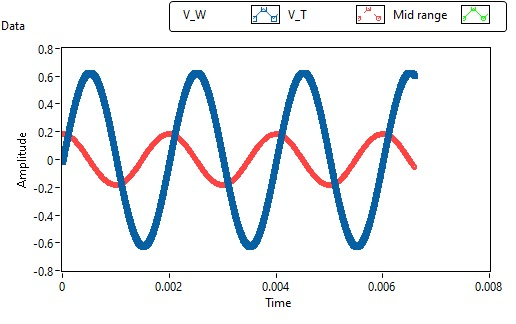
\includegraphics[width=\textwidth]{Cross_waveform_500.jpeg}

\caption{Segnali a 500Hz}
\label{fig:signal_500}

\end{subfigure}

\hfill

\begin{subfigure}[b]{0.3\textwidth}
\centering
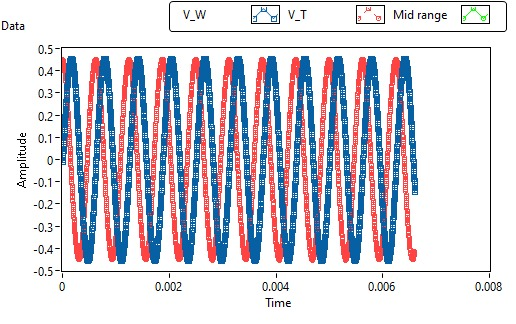
\includegraphics[width=\textwidth]{Cross_waveform_1600.jpeg}

\caption{Segnali a 1600Hz}
\label{fig:signal_1600}

\end{subfigure}

\hfill

\begin{subfigure}[b]{0.3\textwidth}
\centering
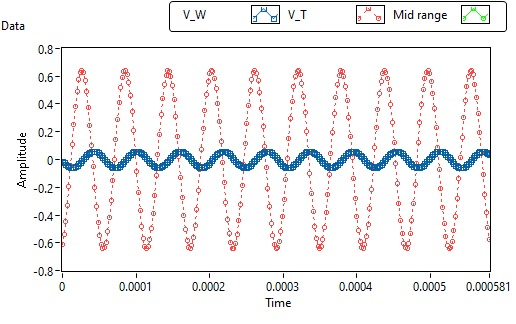
\includegraphics[width=\textwidth]{Cross_waveform_17000.jpeg}

\caption{Segnali a 17kHz}
\label{fig:signal_17k}

\end{subfigure}

\caption{Segnali osservati sui rami Passa-Basso (blu) e Passa-Alto (rosso) a frequenza fissata}
\label{fig:signal_waveforms}

\end{figure}

Dalla figura \ref{fig:signal_waveforms} si nota che 


\subsection{Analisi della frequenza misurata}

\subsection{Analisi dell'ampiezza}

\subsection{Analisi della fase}

\end{document}